\chapter{Анализ современных трактов приема сверхширокополосных сигналов}

Современные тракты приемопередающих устройств сверхширокополосных сигналов широко распространены не только в сфере радиоэлектронной борьбы и разведки, но и в гражданском сегменте. Например, любой современный автомобиль снабжается системами мониторинга дорожной обстановки, помощи водителю и контроля состояния водителя, а также пассажиров. Во многих коммуникационных системах возникает необходимость в определении номера занятого канала (быстрого определения несущей частоты) и т.~п.

Все перечисленные секторы применения электронных устройств, работающих с сверхширокополосными сигналами, объединяет важный аспект, область их применения практически всегда связана с безопасностью человека, поэтому критическим параметром для подобных систем всегда остается быстродействие и низкая вероятность пропуска или ложной тревоги.

Интерес к сверхширокополосным системам растет также благодаря надежде на достижение высоких скоростей обмена информацией по сверхширокополосным беспроводным каналам связи, которые к тому же расположены в нелицензируемых диапазонах частот.

В рамках данной главы будут рассмотрены структуры трактов приемников сверхширокополосных сигналов применяемые в радарах, пеленгаторах и пассивных локаторах.

Сверхширокополосные системы передачи данных находят все более широкое применение \cite{wosbib1}, \cite{vakbib1}, \cite{vakbib2}, \cite{scbib1} в области медицины []-[], организации корпоративных и производственных сетей датчиков []-[], а также [],[] и []...

\section{Структуры современных сверхширокополосных приемных трактов}

Для начала следует дать определение сверхширокополосных сигналов как таковых, что принципиально отличает их от узкополосных сигналов. Сверхширокополосным сигналом называется сигнал, обладающий шириной спектра больше 500 МГц (условно для диапазона частот от 3.1 ГГц до 10.6 ГГц) или же спектральные свойства которого удовлетворяет условию:

\begin{equation*}
\frac{f_H - f_L}{(f_H + f_L)/2} \geqslant 0.25 ,
\label{eq:ubw_condition}
\end{equation*}
где \(f_H\) и \(f_L\) -- верхняя и нижняя границы спектра в пределах которых сконцентрировано не менее 90\% энергии сигнала соответственно.

\fixme{Если при рассмотрении сверхширокополосных сигналов не учитывать время накопления или обработки сигналов, то под понятие сверхширокополосных также попадают сигналы с линейной частотной модуляцией, которые по своей природе таковыми не являются и представляют собой узкополосные сигналы (Ширина спектра порядка нескольких десятков мегагерц) линейно перестраиваемые по частоте. Потому можно выделить две группы сверхширокополосных сигналов, методы приема и обработки которых кардинально различаются.}

Проведен аналитический обзор существующих патентов и коммерческих продуктов с целью создания полноценной классификации существующих систем приема сверхширокополосных сигналов, а также методов повышения быстродействия и помехоустойчивости \cite{jia_4-bit_2020}, \cite{cheng_introduction_2021, lin_60-ghz_nodate, gray_analysis_2009}, \cite{nagulu_ultra-wideband_2021, rahimpour_design_2019, rucker_013m_2009, pelgrom_matching_1989-1, du_112-gss_2019, hartmann_low-power_2007, saha_6-20_2012, johansen_analysis_2005, shahramian_millimeter-wave_2011, du_256-gss_2018, dyskin_wideband_2016, noauthor_photonic_nodate, noauthor_microwave_2005}.

Предложена классификация способов оценки частоты применяемых в современных приемниках индексации частоты, приведенная на рисунке \ref{ct:classification}.

\begin{figure}[ht]
	\centering
	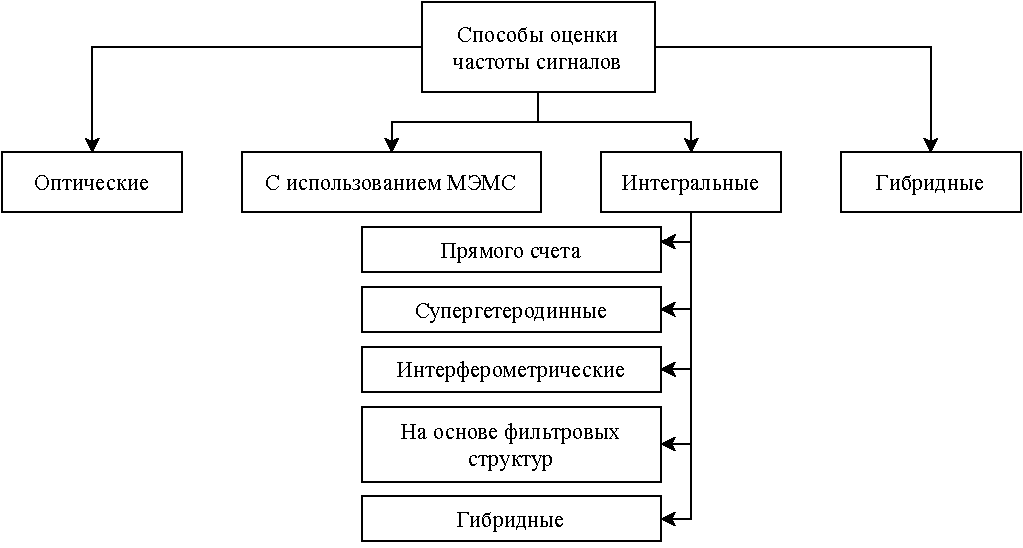
\includegraphics{Classification.pdf}	
	\caption{Классификация способов оценки частоты сверхкоротких импульсов -- pdf\_tex}
	\label{ct:classification}
\end{figure}

\subsection{Супергетеродинные приемники}
Приемники оценки частоты построенные согласно супергетеродинной схеме обладают высокой избирательностью и динамическим диапазоном, что позволяет с высокой точностью [],[] определять частоту сигнала и выполнять идентефикацию источника излучения.

Структурная схема супергетеродинного приемника оценки частоты представлена на рисунке \ref{ct:superhyt}.

\begin{figure}[ht]
	\centering
	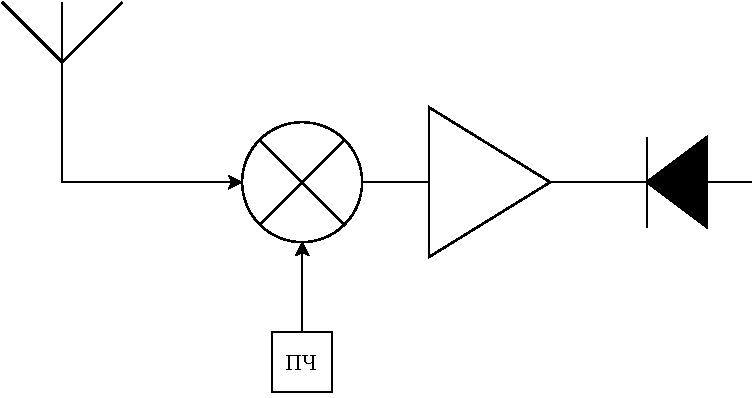
\includegraphics{superhyt.drawio.pdf}	
	\caption{Структурная схема супергетеродинного приемника}
	\label{ct:superhyt}
\end{figure}

\subsection{Приемники прямого преобразования}

\subsection{Приемник измерения мгновенной частоты (IFM)}

Типичная структурная схема приемника измерения (оценки) частоты представлена на рисунке \ref{ct:ifm_struct_simple}. Так как в настоящее время большинство устройств обработки данных принимают данные исключительно в цифровом виде, в данном разделе не будут рассмотренны схемы с аналоговым видеовыходом.

\begin{figure}[ht]
	\centering
	\resizebox{\linewidth}{!}{\input{Dissertation/images/IFM Struct Simple.drawio.pdf_tex}}
	
	\caption{Обобщенная схема простейшего автокорреляционного приемника -- pdf\_tex}
	\label{ct:autocorr_struct_simple}
\end{figure}

\begin{figure}[ht]
	\centering
	\resizebox{\linewidth}{!}{\input{Dissertation/images/IFM Struct Simple.pdf_tex}}
	
	\caption{Структурная схема простейшего приемника измерения мгновенной частоты -- pdf\_tex}
	\label{ct:ifm_struct_simple}
\end{figure}

Измерение частоты в приемнике измерения мгновенной частоты происходит на основе задерживания сигнала в линии задержки (аналоговых электрических, цифровых, оптических) и частотной зависимости разницы фаз задержанного и незадержанного сигналов. Разница фаз вызванная прохождением сигнала через линию задержки описывается выражением \eqref{eq:phase_diff_ifm}.

\begin{equation}
	\theta = \omega \tau ,
	\label{eq:phase_diff_ifm}
\end{equation}
где \(\omega\) и \(\tau\) - частота сигнала и величина линии задержки соответственно.

Для оценки частоты сигнала согласно выражению \eqref{eq:phase_diff_ifm} с известной величиной линии задержки, необходимо измерить разницу фаз сигналов. Для измерения разницы фаз сигналов удобно на выходе приемника представить сигнал в аналитической форме вида \( s(t) = \cos{\theta} + j \sin{\theta} \). Таким образом, выходные сигналы приемника представляются как

\begin{equation}
	\begin{aligned}
		Q &= A \sin{\theta}, \\
		I &= A \cos{\theta}.
	\end{aligned}
	\label{eq:quadrature_ifm}
\end{equation}

Зная величины квадратурных выходных сигналов приемника \(Q\) и \(I\), используя \eqref{eq:atan2_ifm} определяем значение аргумента обоих сигналов.

\begin{equation}
	\theta = \arctan(Q/I) = \omega \tau
	\label{eq:atan2_ifm}
\end{equation}

В соответствии с \eqref{eq:atan2_ifm} находим оценку частоты сигнала как

\begin{equation}
	\omega = \frac{\theta}{2 \pi \tau}.
	\label{eq:ifm_freq_estimation}
\end{equation}

Зависимость оценки частоты сигнала от частоты входного сигнала представлена на рисунке \ref{ct:ifm_out_signal}. Как можно видеть функция имеет периодический характер и прямо пропорционально зависит от величины задержки \(\tau\) (На рисунке \ref{ct:ifm_out_signal} задержка \(\tau \) имеет значение \(400~\textrm{пс}\), что соответствует максимальной индексируемой частоте \(f_{max} = 2.5~\textrm{ГГц}\) ).

\begin{figure}[ht]
	\centering
	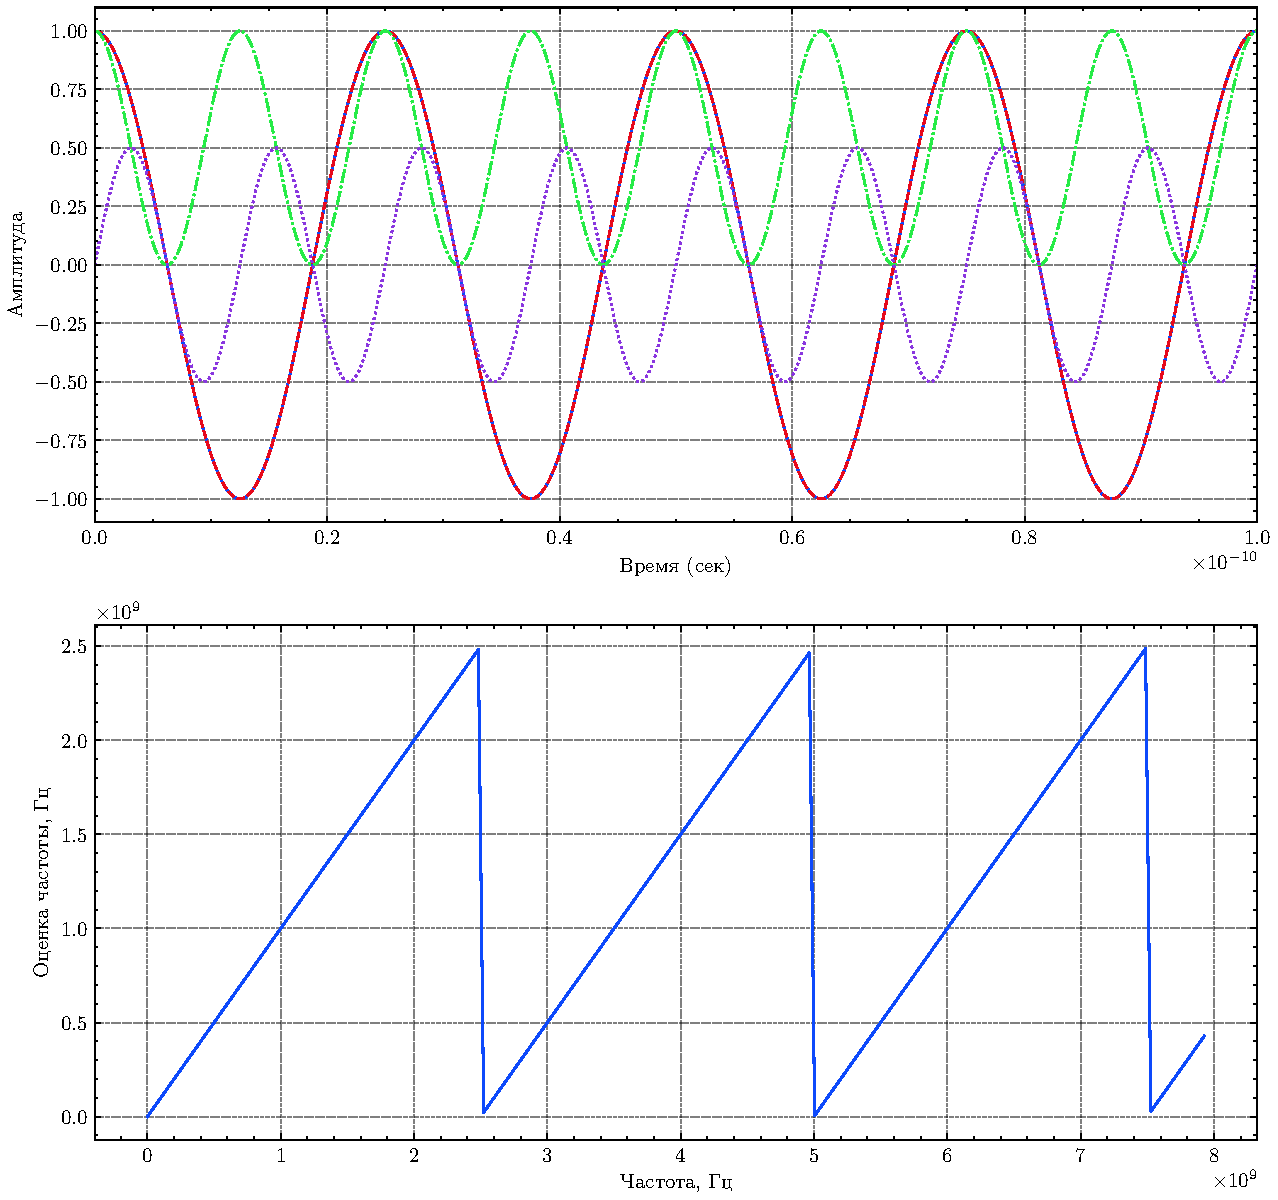
\includegraphics[width=0.6\linewidth]{ifm_out_signal.pdf}
	
	\caption{Выходные сигналы частотного дискриминатора во временной и частотной областях}
	\label{ct:ifm_out_signal}
\end{figure}

Основной проблемой возникающей при использовании приемников МИЧ, является работа при множестве сигналов на входе (два и более). Так как при воздействии на частотный дискриминатор более чем одного сигнала, фазовый сдвиг оцениваемый устройством перестает быть показательным и теряет связь со значением несущей частоты сигналов на входе.

Одним из решений проблемы множественного воздействия на вход приемника, в работе \cite{Choi2014}, \cite{gruchalla_instantaneous_2006}, были представлены структуры многоканальных приемников МИЧ. Разделение на каналы позволяло работать с несколькими сигналами одновременно, однако при этом увеличивается сложность структуры, массо-габаритные характеристики, время проектирования, энергопотребление.

ФРАГМЕНТ ДЛЯ ОПИСАНИЯ ДИСКРИМИНАТОРА С КОМПАРАТОРОМ

Выходное напряжение на выходе дискриминатора описывается выражением
\begin{equation*}
	\begin{aligned}
		V_{q} &= \sin{2 \pi f \tau_{1}},\\
		V_{i} &= \cos{2 \pi f \tau_{1}}.
	\end{aligned}
\end{equation*}

Так как функция \(\sin{x}\) периодична и переходит через ноль с периодом \(\pi\) в точках \(2 f \tau_{1} \in \mathbb{Z} \), возможно путем выбора длины линии задержки устанавливать необходимую частоту перехода дискриминационной характеристики через ноль. Таким образом, установив на выходе частотного дискриминатора компаратор, можно идентифицировать и исключать зоны неоднозначности при оценке частоты в широком диапазоне частот.

Для устранения неоднозначности оценки частоты в широком диапазоне частот необходим правильный выбор величины линии задержки, т.к. при задерживании сигнала больше необходимого, дискриминационная характеристика \(V_s\) будет изменять знак более одного раза в рабочем диапазоне частот. Величина линии задержки выбирается таким образом, что
\begin{equation*}
	BW < \frac{1}{2 \tau_{1}}.
\end{equation*}

\todo{12sdasds}

\note{asdsadasd}

\subsection{Приемник прямого счета}
Патент \textbf{US5337051} описывает систему оценки частоты сигналов на основе прямого счета изменений знака входного сигнала (Zero Crossing) и линейной аппроксимации момента времени в который сигнал приблизительно равен нулю. Структурная схема представлена на рисунке~\ref{ct:zerocross_struct}.
\begin{figure}[ht]
	\centering
	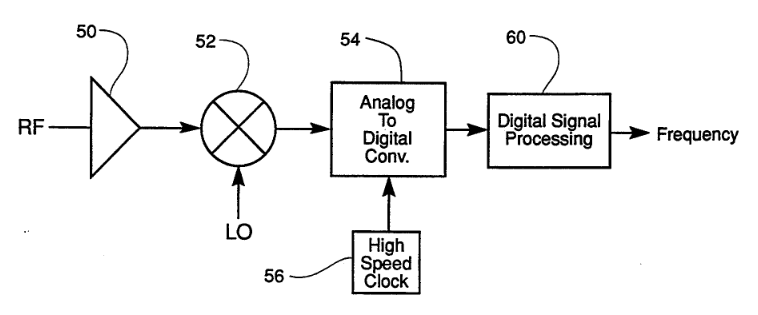
\includegraphics[width=0.6\linewidth]{zerocross_struct}
	
	\caption{Структурная схема частотного дискриминатора на основе счета пересечений нуля и линейной аппроксимации}
	\label{ct:zerocross_struct}
\end{figure}

\begin{figure}[ht]
	\centering
	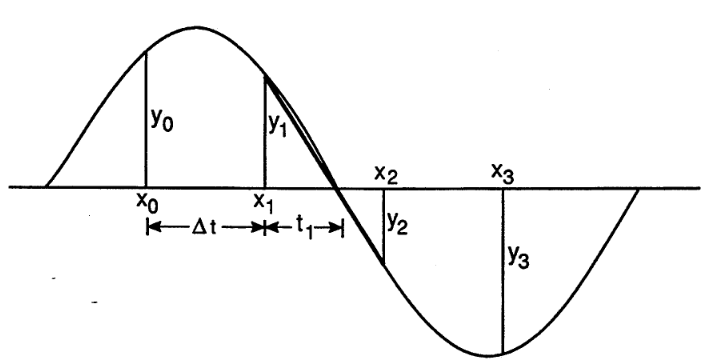
\includegraphics[width=0.6\linewidth]{zerocross_time}
	
	\caption{Временная диаграмма, описывающая принцип работы частотного дискриминатора на основе счета пересечений нуля и линейной аппроксимации}
	\label{ct:zerocross_time}
\end{figure}

\subsection{Компрессионный приемник (Compressive sensing)}

\subsection{Прочие и гибридные виды приемников}

\subsection{Выводы по разделу}

На основании проведенного анализа различных структур приемников измерения мгновенной частоты ...
Результаты анализа сведены в таблицу \ref{t:survey}, в которой отражены ключевые характеристики различных приемников.

\begin{table}
\caption{Сравнение характеристик приемников измерения мгновенной частоты\label{t:survey}}
	\begin{adjustbox}{width=\columnwidth,center}
		
		\begin{tabular}{@{}m{8em}cccccc@{}}
			\toprule
													&	Супергетеродинный	& Многоканальный & МИЧ & Компрессионный & Оптический & Детекторный\\
			\midrule
			Ширина рабочей полосы					&	Хуже 				& Хорошо	& Превосходно	& Хорошо & Хорошо & Превосходно\\
			Стойкость к множеству сигналов на входе &	Хуже 				& Хорошо	& Хуже	& Хорошо & Хорошо & Хуже\\
			Разрешение по частоте 					& 	Превосходно 		& Хорошо	& Хорошо	& Хорошо & Хорошо & Хуже\\
			Чувствительность 						& 	Превосходно 		& Хорошо	& Умеренно	& Хорошо & Умеренно & --\\
			Динамический диапазон 					& 	Превосходно 		& Хорошо	& Умеренно	& Умеренно & Хуже & Умеренно\\
			Быстродействие							&	Умеренно			& Умеренно	& Превосходно & Хуже	& Умеренно & Превосходно \\
			\bottomrule
		\end{tabular}
	\end{adjustbox}
\end{table}

\section{Особенности реализации систем оценки частоты в интегральном исполнении}

\subsection{Применение искусственных линий задержки}
Работ по применению искусственных линий задержек в сверхширокополосных системах на кристалле сравнительно немного. Исследованиями в данной области занимаются такие ученые как ...

Применение искусственных линий задержки обусловлено необходимости уменьшения площади топологии микросхемы, избежание проблем с электромагнитной совместимостью, а также как будет показано в данном разделе для обеспечения необходимых частотных характеристик многоканальной системы.

Главным образом искусственной линией задержки называется такая структура из сосредоточенных или распределенных компонентов, которая в определенных условиях повторяет поведение физической линии передачи, например LC-звено на сосредоточенных элементах, в определенном диапазоне частот, соответствует с точки зрения вносимого сдвига фаз длиной коаксиальной или микрополосковой линии.

\begin{equation*}
	\begin{aligned}
		\frac{\partial v(z,t)}{\partial z}
	\end{aligned}
\end{equation*}

\subsection{Динамический диапазон}


\section{Принципы и методы оценки быстродействия сверхширокополосных систем}

\subsection{Понятие быстродействия, метрика и т.п.}

\section{Принципы действия и характеристики современных трактов приема сверхширокополосных импульсных сигналов}

\section{Главный тракт приема сверхширокополосных сигналов с точки зрения назначения и применения}
Главный тракт приема в радиочастотных системах выполняет функции преселекции и усиления сигналов в необходимой полосе частот. Из расположения главного тракта в структуре приемной аппаратуры и выполняемых функций становится очевидно его доминирующее влияние на производительность всей системы в целом.

Проблемы проектирования трактов приема сверхширокополосных сигналов в интегральном исполнении активно обсуждаются на протяжении последних Х лет, такими авторами как ...

Наиболее широкое распространение получили приемопередатчики на основе сигналов с прямым расширением спектра, сигналов с псевдослучайной перестройкой по частоте, а также импульсное радио с скачками по времени. Из вышеперечисленных, большинство работ посвящено структурам, работающим с импульсными сигналами, как схемам с наиболее выгодной практической реализацией. Импульсное радио позволяет получить приемлемую скорость передачи данных, возможность определения расстояния и  местоположения объектов в пространстве, а также простую реализацию устройства с малым энергопотреблением [], [] и [].

\subsection{Высокоскоростные сети обмена информацией}

\subsection{Низкоскоростные сети (Сети датчиков, сенсоров или вещей)}

\subsection{Устройства распознавания образов}

\subsection{Устройства определения параметров объектов (Радары)}
Приемники предназначенные для определения параметров принимаемых сигналов значительно отличаются от информационных приемников. Информационные приемники предназначены для восстановления иннформации передаваемой передатчиком. Приемники сигналов радаров не восстанавливают передаваемую информацию, а определяют такие характеристики сигнала, как ширина импульса, форма, частота, частота следования импульсов и угол прихода сигнала (Angle of Arrival).

Исходя из специфики выполняемых задач, подобные приемники должны удовлетворять следующим требованиям:
\begin{itemize}
\item Широкий частотный диапазон;

\item Высокая чувствительность и динамический диапазон;

\item Быстродействие обработки и идентификации характеристик принимаемых сигналов;

\item Возможность обработки двух и более сигналов одновременно;

\item Устойчивость к внешним воздействиям (Широкий температурный диапазон, высокая входная мощность, стойкость к ионизирующему излучению).
\end{itemize}

 Следует также подчеркнуть причину по которой подходы к проектированию связных сверхширокополосных приемников и приемников обнаружения сверхкоротких импульсов (а также оценки их характеристик) так сильно различаются. При проектировании связного приемника и в целом приемо-передающего тракта, параметры и характеристики передаваемых сигналов заранее определены, известны спектральные свойства сигналов несущих информацию.
 В то же время, проектирование приемника обнаружения сверхкоротких импульсов не может осуществляться по тем же методам, что и связные, так как принимаемые сигналы заведомо неизвестны, отсутствует какая-либо синхронизация на приеме и передаче и самое важное, отсутствует цель как таковая прием информационных сообщений. Зондирующие импульсы радарных систем не несут в себе какой-либо информации, информацией для принимающей стороны является сам факт детектирования сигналов данного вида, определения их принадлежности, направления излучения.

\section{Выводы по разделу}